% rubber: set program xelatex
\documentclass[a4paper,12pt]{article}

\usepackage{xltxtra}
\usepackage{amsmath,amsthm,amssymb}

\usepackage[autostyle=true]{csquotes}
\usepackage{polyglossia}
\setmainlanguage[variant=mono]{greek}
\setotherlanguage{english}

% Fonts
\setmainfont{CMU Serif}                 
\setsansfont{CMU Sans Serif}            
\setmonofont{CMU Typewriter Text}


\usepackage[margin=1in]{geometry} 

% Source code listings
\usepackage{listings}
\usepackage{color}
\lstset{language=C++,basicstyle=\ttfamily\small, keywordstyle=\color{blue}\ttfamily,
        stringstyle=\color{red}\ttfamily,  commentstyle=\color{magenta}\ttfamily,
        showstringspaces=false, numbers=none, morecomment=[l][\color{green}]{\#}}

% Disable paragraph intention 
\setlength\parindent{0pt}  

\usepackage{multicol} 

\begin{document}
\title{Data Structured and Algorithms\\ Msc Program 2017-2018}
\author{Giannis Tsagatakis\\
4\textsuperscript{th} Assignment: Graphs} 
 
\maketitle

\section*{R-6.4}
Bob loves foreign languages and wants to plan his course schedule to take
the following nine language courses: LA15, LA16, LA22, LA32, A126, LA127,
LA141, LA169. Given the course prerequisities, find a sequence of courses that allows Bob to satisfy all the prerequisities.
\begin{figure}[h] 
	\centering
	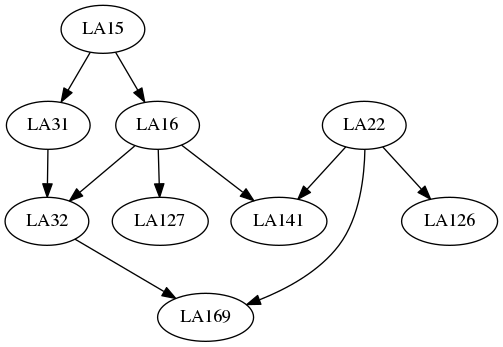
\includegraphics[width=8cm]{code/gcourses.png} 
	\caption{Course prerequisites}	 
\end{figure}


\subsection*{Solution}
Solution using the topological sorting algorithm. 
\begin {itemize} 
\item First we build a digraph to represent the course prerequisite requirements. 
\item Then apply the topological sorting algorithm on the graph.
\end {itemize}

\subsubsection*{Implementation}
\lstinputlisting[linerange={1-25}]{code/topSort.cpp}
\begin{figure} 
	\centering
	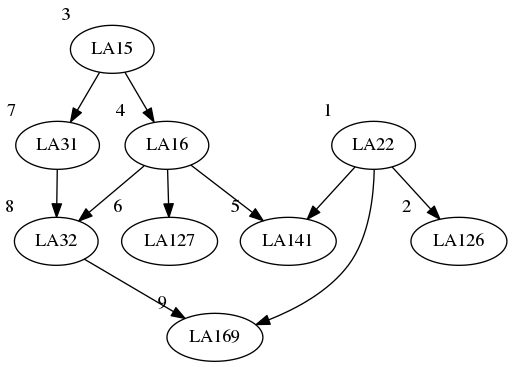
\includegraphics[width=8cm]{code/gcourses-solution.png} 
	\caption{Course prerequisites solution.}	 
\end{figure}
\lstinputlisting[linerange={26-200}]{code/topSort.cpp}

\subsection*{Coding solution} 
\begin{verbatim}
Topological Sort:
LA22 -> LA126 -> LA15 -> LA16 -> LA141 -> LA127 -> LA31 -> LA32 -> LA169
\end{verbatim}

%%%%%%%%%%%%%%%%%%%%%%%%%
%%%%%%%%%%%%%%%%%%%%%%%%%
%%%%%%%%%%%%%%%%%%%%%%%%%

\section*{R-6.6}
Let G be a graph whose vertices are the integers 1 through 8, and let the adjacent vertices
of each vertex be given by the table given as code below:

\begin{multicols}{3}
\lstinputlisting[linerange={106-131}]{code/DFS.cpp}
\end{multicols}

Assume that, in a traversal of G, the adjacent vertices of a given vertex are returned in the
same order as they are listed in the above table.
\begin {itemize} 
\item Draw G. 
\item Order the vertices as they are visited in a DFS traversal starting at vertex 1.
\item Order the vertices as they are visited in a BFS traversal starting at vertex 1.
\end {itemize}


\subsection*{DFS Implementation}
The solution share alot of code with the previous algorithm. The code is a bit more simple actually. A list is used to hold the visited nodes instead of a stack. Thus only the most important parts of the alogorithm is given bellow.
\begin{figure} 
	\centering
  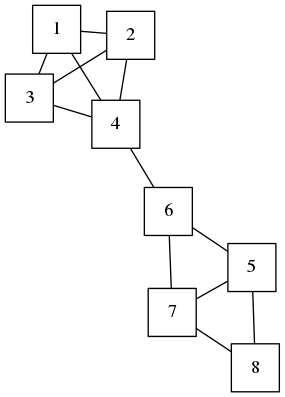
\includegraphics[width=4cm]{code/DFS.png}	
	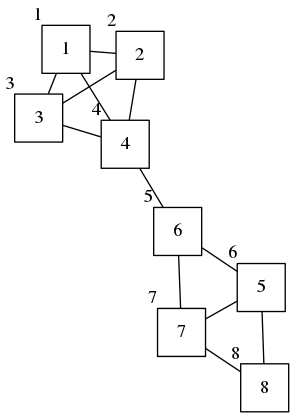
\includegraphics[width=4cm]{code/DFS-solution.png}
	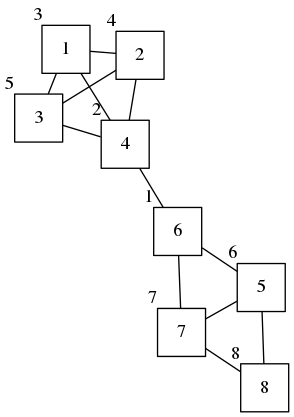
\includegraphics[width=4cm]{code/DFS-solution2.png} 
	\caption{2 Solutions and the original problem.}	 
\end{figure}

% Driver
\lstinputlisting[linerange={69-82}]{code/DFS.cpp} 
%__dfs__Sort
\lstinputlisting[linerange={91-100}]{code/DFS.cpp} 
\lstinputlisting[linerange={146-156}]{code/DFS.cpp}

Test run
\lstinputlisting[linerange={135-141}]{code/DFS.cpp}

\subsection*{DFS Coding solution}
\begin{verbatim}
DFS Sort starting from :1
1->2->3->4->6->5->7->8

DFS Sort starting from :6
6->4->1->2->3->5->7->8) 
\end{verbatim} 

\section*{R-6.10}
Compute a topological ordering for the directed graph drawn with solid
edges in Figure.

\subsection*{Flight Implementation}
The code is the almost the same as the 1st exersize.
\lstinputlisting[linerange={48-70}]{code/topoSort610.cpp} 

\begin{figure} 
	\centering
	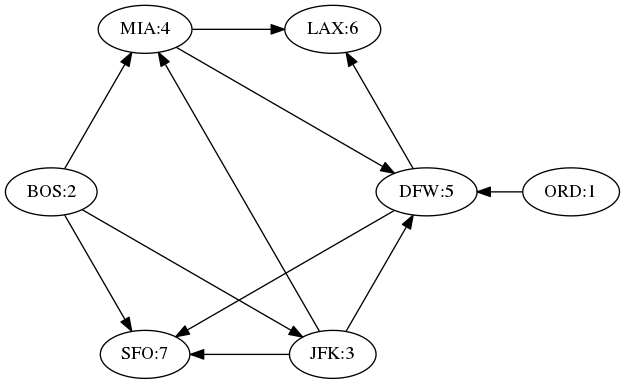
\includegraphics[width=12cm]{code/gflights-solution.png}
	\caption{Topological Sort of the flights problem.}	 
\end{figure}

The driver program.
\lstinputlisting[linerange={128-159}]{code/topoSort610.cpp} 


\subsection*{Flight Coding solution}
\begin{verbatim}
Topological Sort:
ORD -> BOS -> JFK -> MIA -> DFW -> LAX -> SFO
\end{verbatim}



\section*{R-6-7}
Would you use the adjacency list structure or the adjacency matrix
structure in each of the following cases? Justify your choice.

\subsection*{Solution}
 \begin {enumerate} 
 
 \item The graph has 10,000 vertices and 20,000 edges, it is important to use as little space as possible
 
 The adjacency matrix needs space of $10,000 \times 10,000 = 100,000$ elements for a directed graph and the half for an undirected graph. The adjacency list structure needs only storage for $20,000$ edge elements (the data and the pointers). Clearly the adjacency list structure is preferable in this case. 
 
 \item The graph has 10,000 vertices and 20,000,000 edges, and it is important to use as little space as possible.
 
 There is no clear winner here. The exact space requirements depends on immplementation details like the size of a pointer. In this case it will be better if we use criteria like the next question to decide.
 
\item You need to answer the query \texttt{areAdjecent} as fast as possible, no matter how
much space you use.
 
 The adjacency matrix structure is much better for operation \texttt{areAdjacent }, while the adjacency list structure is much better for operations \texttt{insertVertex } and \texttt{removeVertex }. Clearly here the adjacency matrix structure is preferable. Indeed, it supports operation \texttt{areAdjacent } in $O(1)$ time, irrespectively of the number of vertices or edges. 

\end {enumerate} 
 

\section*{R-6-9}
Draw the transitive closure of the directed graph shown in Figure

\subsection*{Transitive closure Implementation}
\lstinputlisting{code/transitive.cpp}

\begin{figure} 
	\centering
  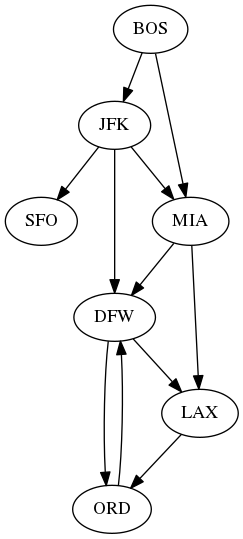
\includegraphics[width=3.5cm]{code/gflight.png}	
	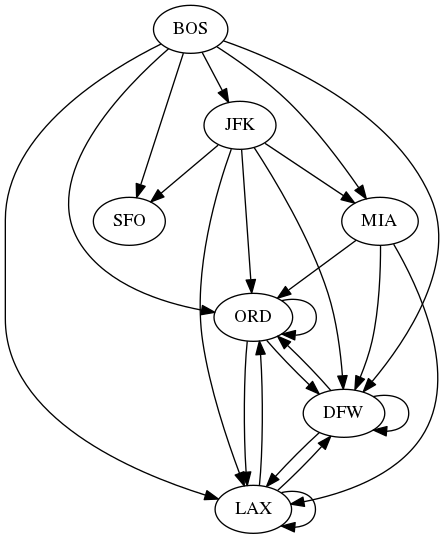
\includegraphics[width=6cm]{code/gflight-trans.png} 
	\caption{The transitive close of the flights problem.}	 
\end{figure}
 
\begin{center}
 \begin{tabular}{||c | c c c c c c c c||} 
 \hline
%%%%%%%%%
	&SFO	&BOS	&ORD	&JFK	&DFW	&LAX	&MIA	&\\
\hline\hline
SFO	&0		&0		&0		&0		&0		&0		&0		&\\
BOS	&1		&0		&1		&1		&1		&1		&1		&\\
ORD	&0		&0		&1		&0		&1		&1		&0		&\\
JFK	&1		&0		&1		&0		&1		&1		&1		&\\
DFW	&0		&0		&1		&0		&1		&1		&0		&\\
LAX	&0		&0		&1		&0		&1		&1		&0		&\\
MIA	&0		&0		&1		&0		&1		&1		&0		&\\
%%%%%%%
\hline
\end{tabular}
\end{center}

\vfill
\noindent Tools used: \texttt{clang++}, \texttt{clion},  \texttt{cmake}, \LaTeX{}, \texttt{clang-format}, \texttt{graphviz dot}.
\end{document}
